\documentclass[11pt]{article}

\usepackage[margin=1in]{geometry}
\usepackage{graphicx}
\usepackage{amsmath}
\usepackage{amssymb}
\usepackage{float}
\usepackage{hyperref}
\usepackage{natbib}

\title{Evaluating Persona Libraries Against Revealed Human Behavior}
\author{Robin Na}
\date{\today}

\begin{document}
\maketitle

\begin{abstract}
Persona prompting is increasingly used to simulate heterogeneous human populations with large language models. The central assumption is that a textual persona can be transferred into appropriate behavior in a new environment. We propose a direct evaluation of that transfer step. Rather than asking a model to generate actions, we show it completed human interactions and ask which observed player best matches a persona. This lets us measure whether a persona-library-plus-model system covers the revealed behavioral support of a target study, choosing among real human trajectories instead of generating its own actions.

Using direct Twin persona summaries, we apply this evaluation in public goods games and chip bargaining. In both settings, top-1 choices are more concentrated than expected under a request-conditional uniform null. Public goods games show the stronger failure profile: many observed player identities are never selected and matched players are systematically more cooperative, more rewarding, and less punished. Chip bargaining shows broader identity coverage, but still significant concentration and a bargaining-specific skew toward players with more successful accepted proposals. These results suggest that source-space persona diversity can compress into narrowed and behaviorally skewed target-action coverage.
\end{abstract}

\section{Motivation}

LLMs are increasingly used to simulate human respondents, strategic agents, and synthetic populations. Prior work has shown that models can sometimes reproduce survey patterns, experimental results, or subgroup differences when conditioned on demographic or persona prompts \citep{argyle2023silicon,aher2023turing}. More recent benchmarks and agent-based simulations extend this idea to richer behavioral settings \citep{hu2025simbench,park2023generative,vezhnevets2023concordia}.

The problem is that a persona is not a behavioral policy. It is a text description that a model must translate into action in a new environment. A persona that appears diverse or realistic in its source domain may map, through the model, to a much narrower region of target behavior. Existing rollout evaluations conflate two issues: whether the persona library contains the relevant behavioral types, and whether the model can calibrate generated actions. Our evaluation isolates the first issue as much as possible by asking the model to choose among real human trajectories, instead of generating its own actions.

\section{Evaluation Design}

For each request, the model receives one persona summary and one observed game transcript. It returns up to three observed players with probabilities summing to one. We use a ranking and probability-allocation task because the target question is not whether the model can invent a calibrated contribution path, punishment decision, or bargaining proposal. The target question is whether the persona, as interpreted by the model, maps onto the kinds of people who actually appeared in the target environment. Ranking real participants makes the test intentionally easier than rollout simulation: the model only needs to identify which revealed trajectory the persona could most plausibly have produced.

Formally, let \(p \in \mathcal{P}\) index persona summaries and \(g \in \mathcal{G}\) index observed games. Each game \(g\) contains a candidate set of human players \(C_g=\{1,\ldots,J_g\}\), each with a revealed trajectory \(T_{gj}\) that includes actions and, when available, communication. A request \(r=(p,g)\) asks the model to return a sparse probability vector over the candidates:
\[
q_r \in \Delta(C_g), \qquad q_{rj}\ge 0,\qquad \sum_{j\in C_g} q_{rj}=1,\qquad |\{j:q_{rj}>0\}|\le 3.
\]
The top-1 match is
\[
m_r=\arg\max_{j\in C_g}q_{rj}.
\]
The estimand is not a generated action distribution. It is the distribution over observed human trajectories induced by the persona-library-plus-model mapping, \(F:(p,T_g)\mapsto q_r\).

We evaluate this mapping with three diagnostics. Local concentration asks whether many personas select the same observed player within a fixed game. Global identity collapse asks whether top-1 mass covers too few observed people across the full target corpus. Behavioral skew asks whether matched players are systematically different from the candidate players shown in the same requests.

Local concentration is evaluated within each game by counting how many personas select each player as the top-1 match:
\[
n_{gj}=\sum_{r:g(r)=g}\mathbf{1}\{m_r=j\}, \qquad
L_g=\frac{\max_{j\in C_g}n_{gj}}{N_g}, \qquad
N_g=\sum_{j\in C_g}n_{gj}.
\]
The within-game null is
\[
m_r \overset{H_0}{\sim} \mathrm{Uniform}(C_g)
\]
independently across requests for the same game. We use this null both to simulate 95 percent intervals for \(L_g\) and to test whether the vector \((n_{g1},\ldots,n_{gJ_g})\) is distinguishable from a uniform multinomial distribution. We apply Benjamini-Hochberg correction across games within each target environment.

Global identity collapse is evaluated by aggregating top-1 choices over all successful requests. Let \(I\) be the set of candidate identities that appear in at least one request and \(s_i=n_i/\sum_i n_i\) be identity \(i\)'s share of top-1 selections. We compute selected-identity share \(S\), normalized entropy effective number \(E\), and top-5 percent identity mass \(M_{0.05}\):
\[
S=\frac{|\{i\in I:n_i>0\}|}{|I|}, \qquad
E=\frac{\exp\left(-\sum_i s_i\log s_i\right)}{|I|}, \qquad
M_{0.05}=\sum_{i\in \mathrm{Top}_{0.05}(I)}s_i.
\]
The request-conditional uniform null redraws \(m_r\) uniformly from the exact candidate set \(C_{g(r)}\) shown in request \(r\), preserving the number of personas, games, requests, and candidate players per game. We compare observed statistics with 20,000 draws from this null.

Behavioral skew is evaluated at the request level. For a behavior metric \(Y_{gj}\), the probability-weighted matched value is compared with a candidate-uniform baseline over the players shown in the same transcript:
\[
\Delta_Y
=\frac{1}{R}\sum_r\left[
\sum_{j\in C_{g(r)}}q_{rj}Y_{g(r)j}
-\frac{1}{J_{g(r)}}\sum_{j\in C_{g(r)}}Y_{g(r)j}
\right].
\]
We plot \(\Delta_Y\) divided by the candidate-uniform standard deviation of \(Y\). PGG uncertainty intervals use game-cluster bootstraps; chip-bargaining intervals use record-cluster bootstraps.

\section{Results}

\begin{figure}[H]
\centering
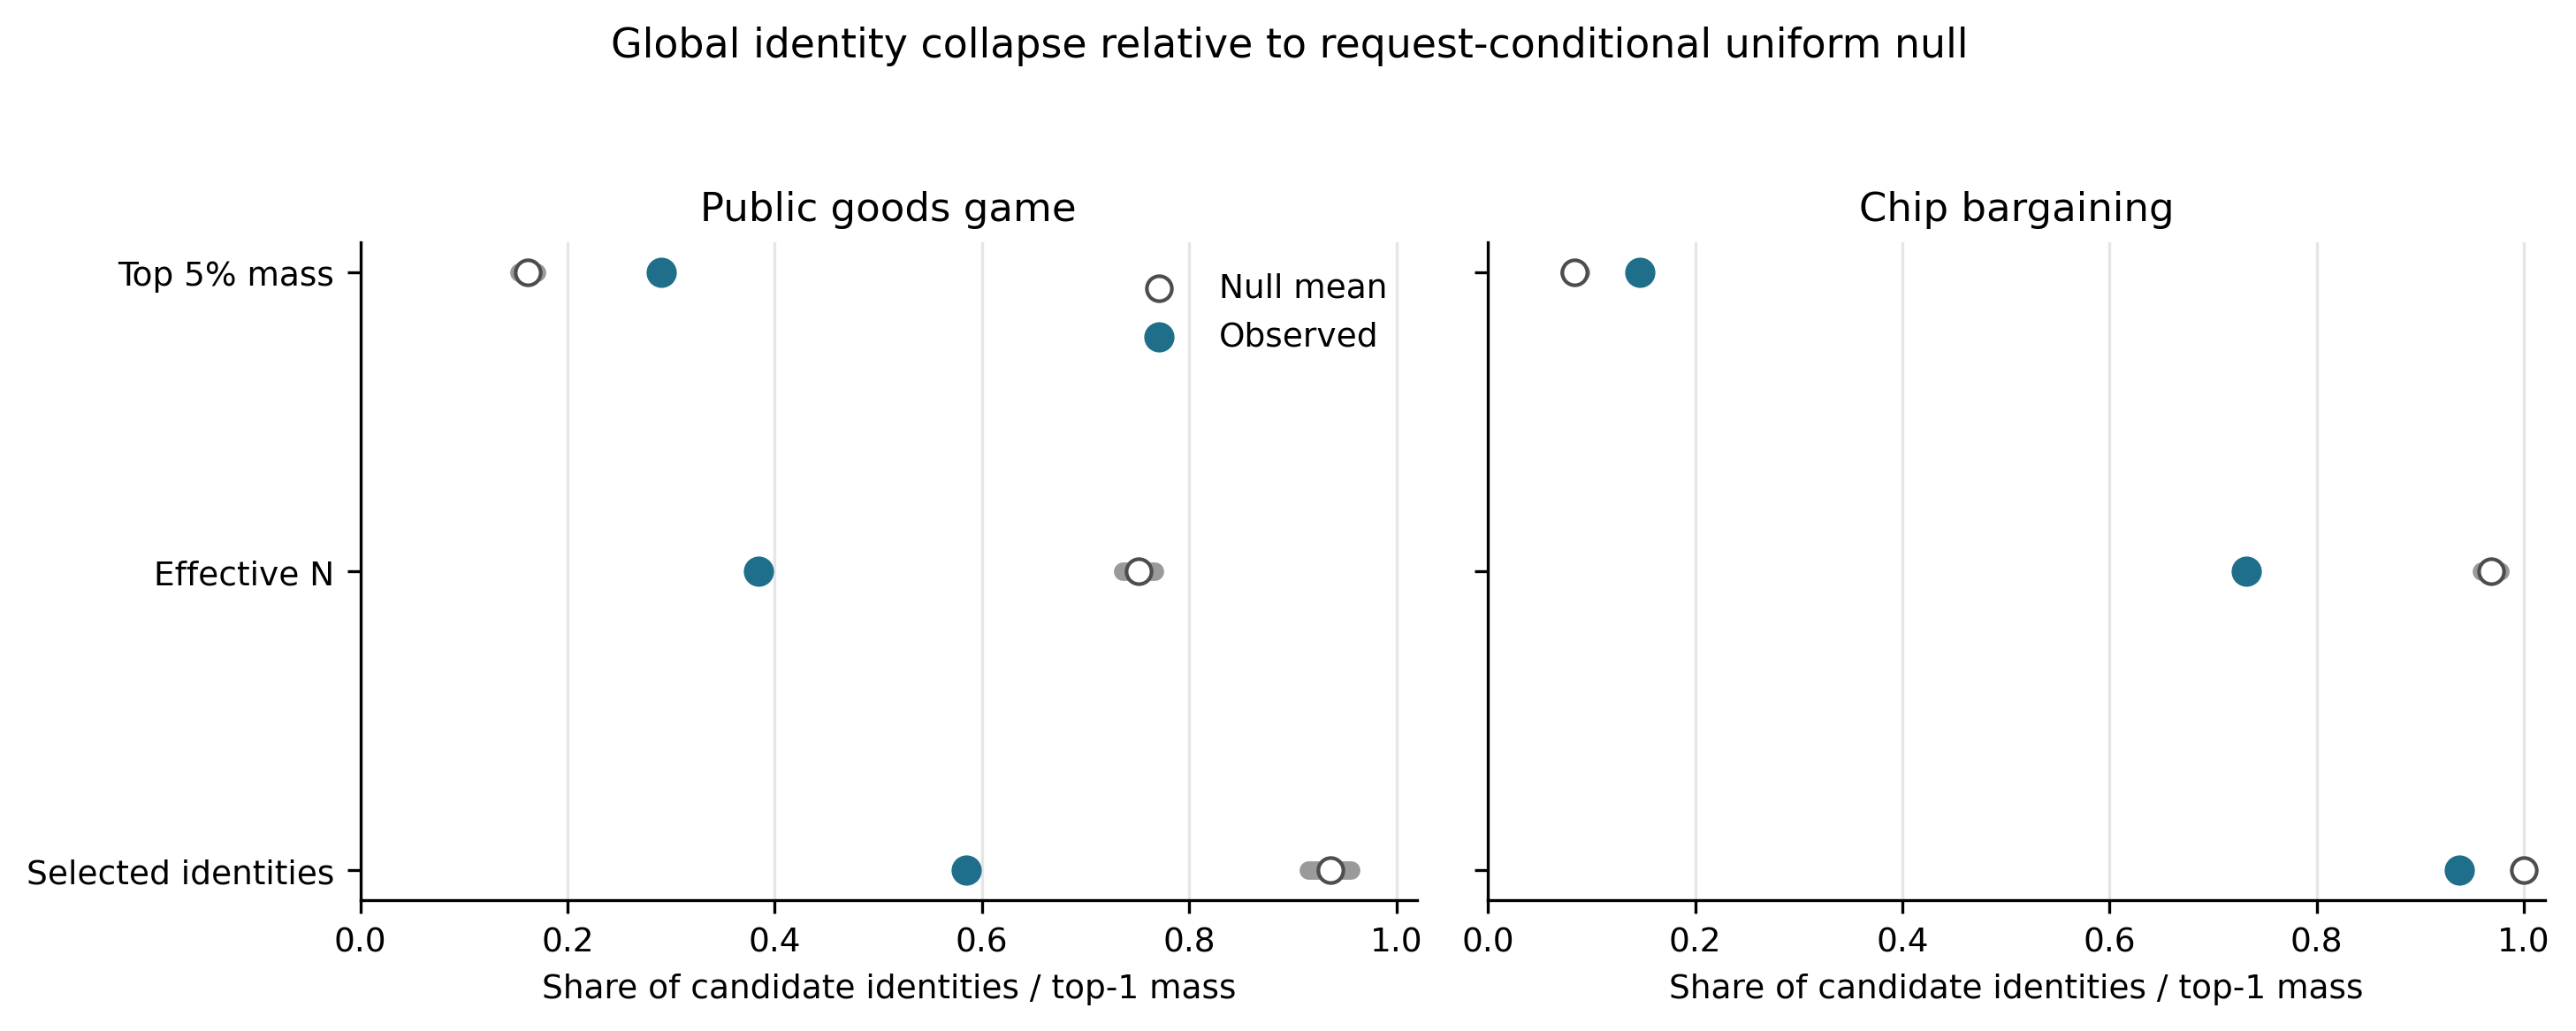
\includegraphics[width=\linewidth]{../figures/figure_global_identity_collapse.png}
\caption{\textbf{Global identity collapse relative to a request-conditional uniform null.} For each successful request, the null redraws the top-1 match uniformly from the players shown in that request, preserving the number of personas, games, and candidate players per game. Gray intervals show 95 percent simulation intervals from 20,000 null draws, open circles show null means, and filled circles show observed values. Selected identities and effective \(N\) are normalized by the number of candidate identities; top 5 percent mass is the share of all top-1 selections received by the most-selected 5 percent of observed identities.}
\label{fig:global-collapse-short}
\end{figure}

\begin{figure}[H]
\centering
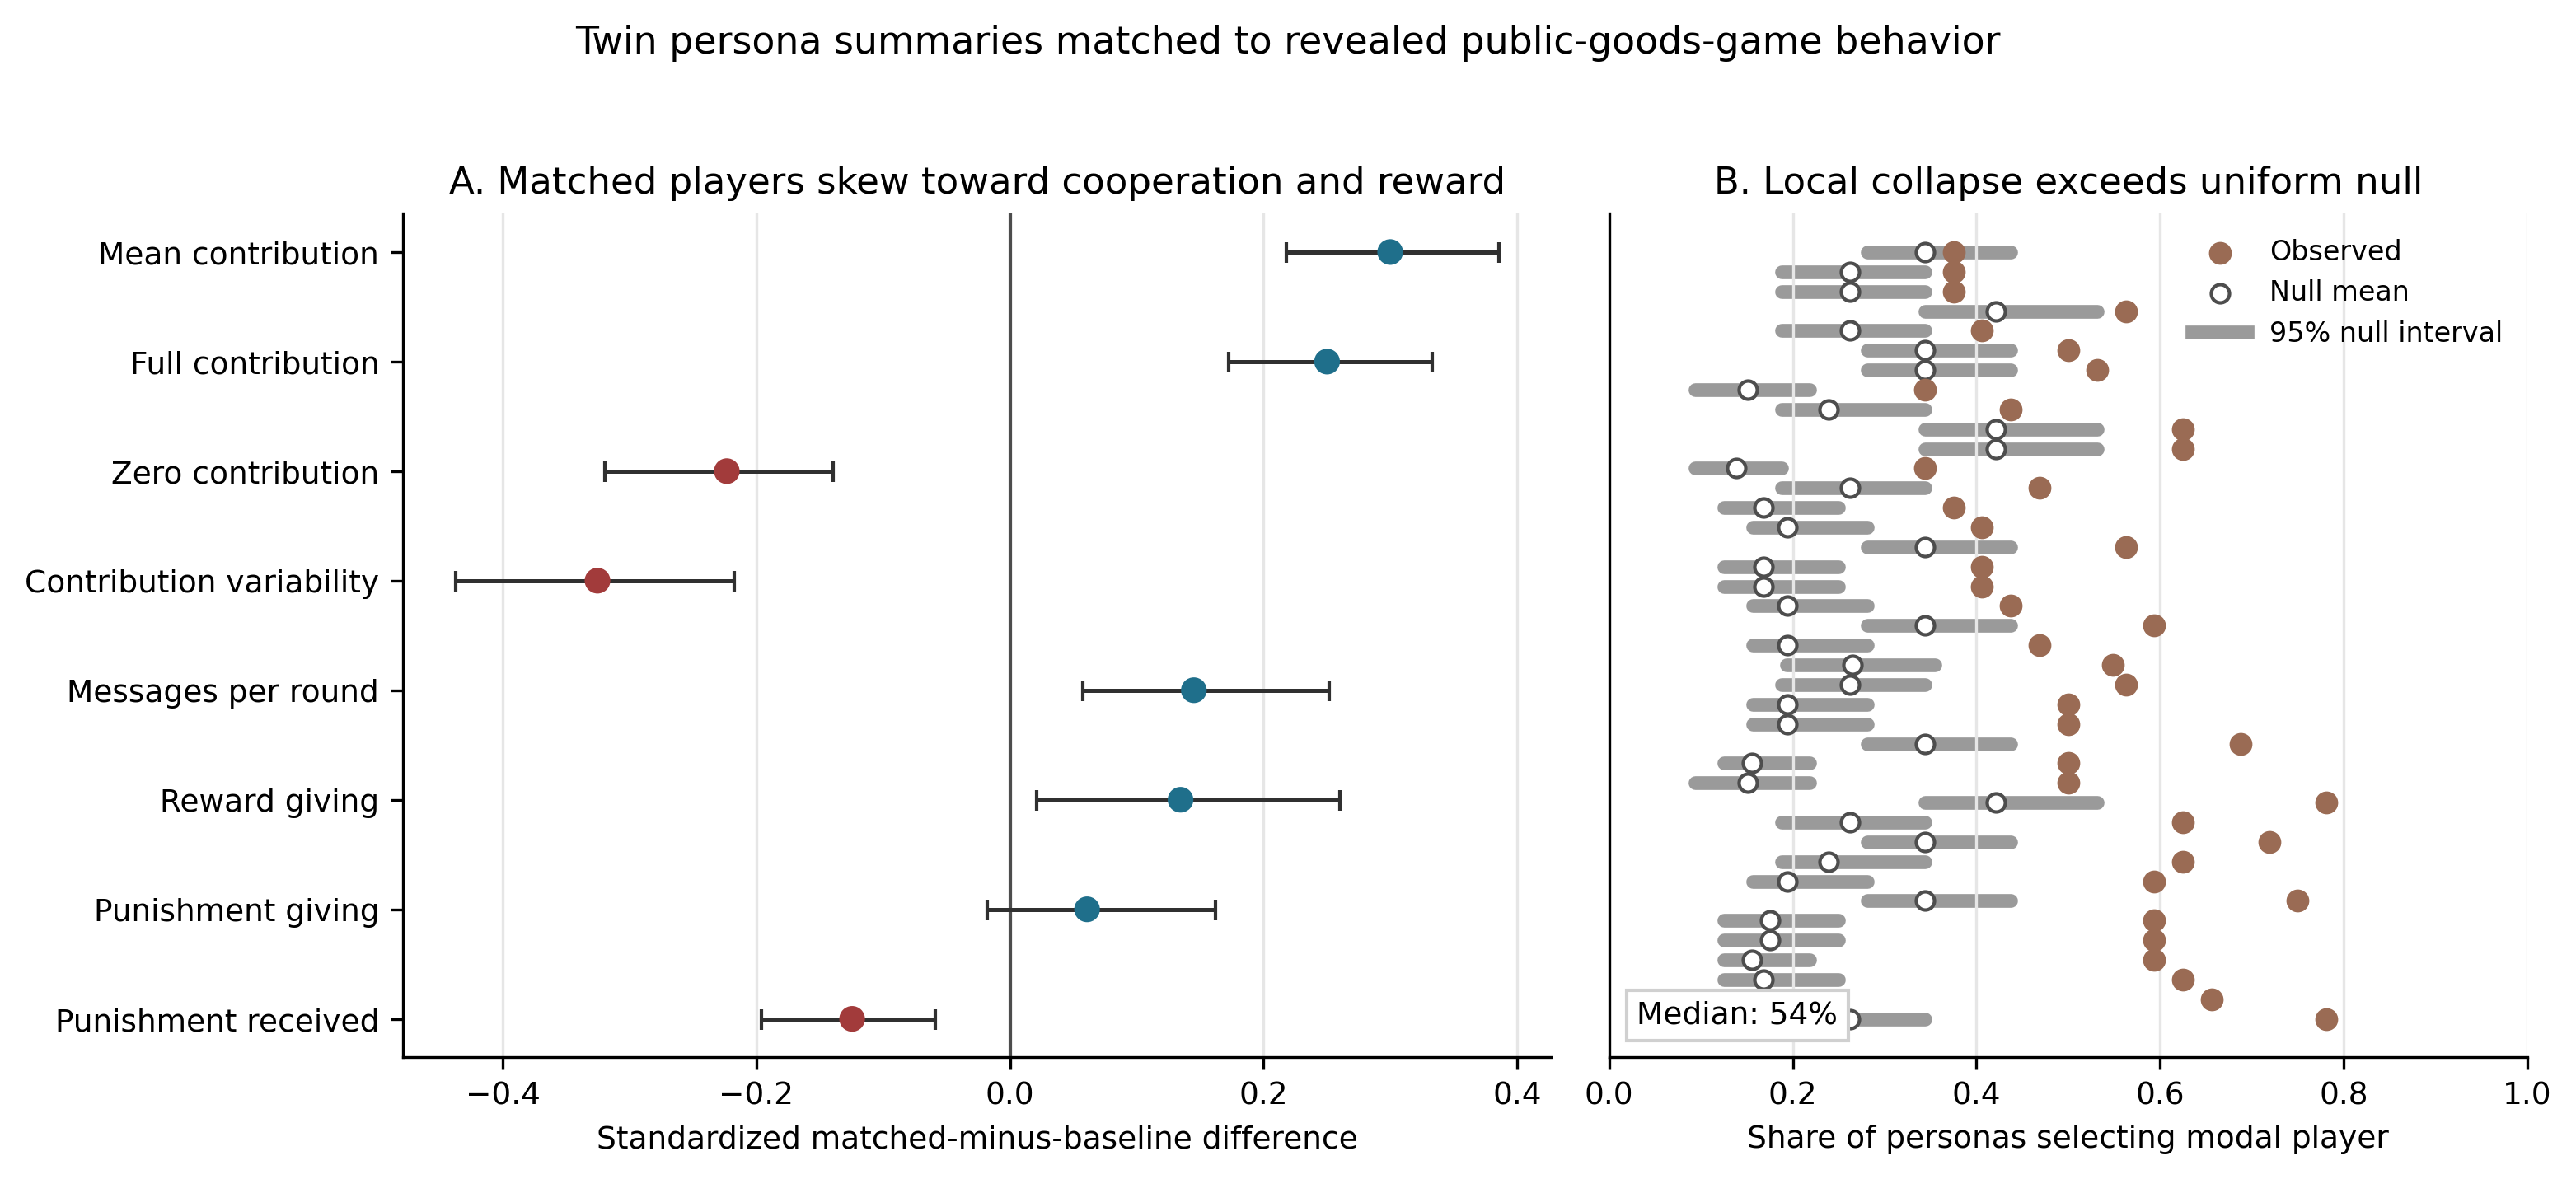
\includegraphics[width=\linewidth]{../figures/figure_pgg_behavior_local_collapse.png}
\caption{\textbf{Public-goods-game transfer evaluation.} Panel A reports probability-weighted matched-minus-candidate-uniform differences, divided by the candidate-uniform standard deviation for each behavior metric. Error bars are 95 percent game-cluster bootstrap intervals. Panel B reports local concentration against the within-game uniform null: for each fixed game transcript, filled points show the observed modal top-1 share across personas, open points show the null mean, and gray intervals show 95 percent null intervals from uniform top-1 selection over the players in that game.}
\label{fig:pgg-short}
\end{figure}

\begin{figure}[H]
\centering
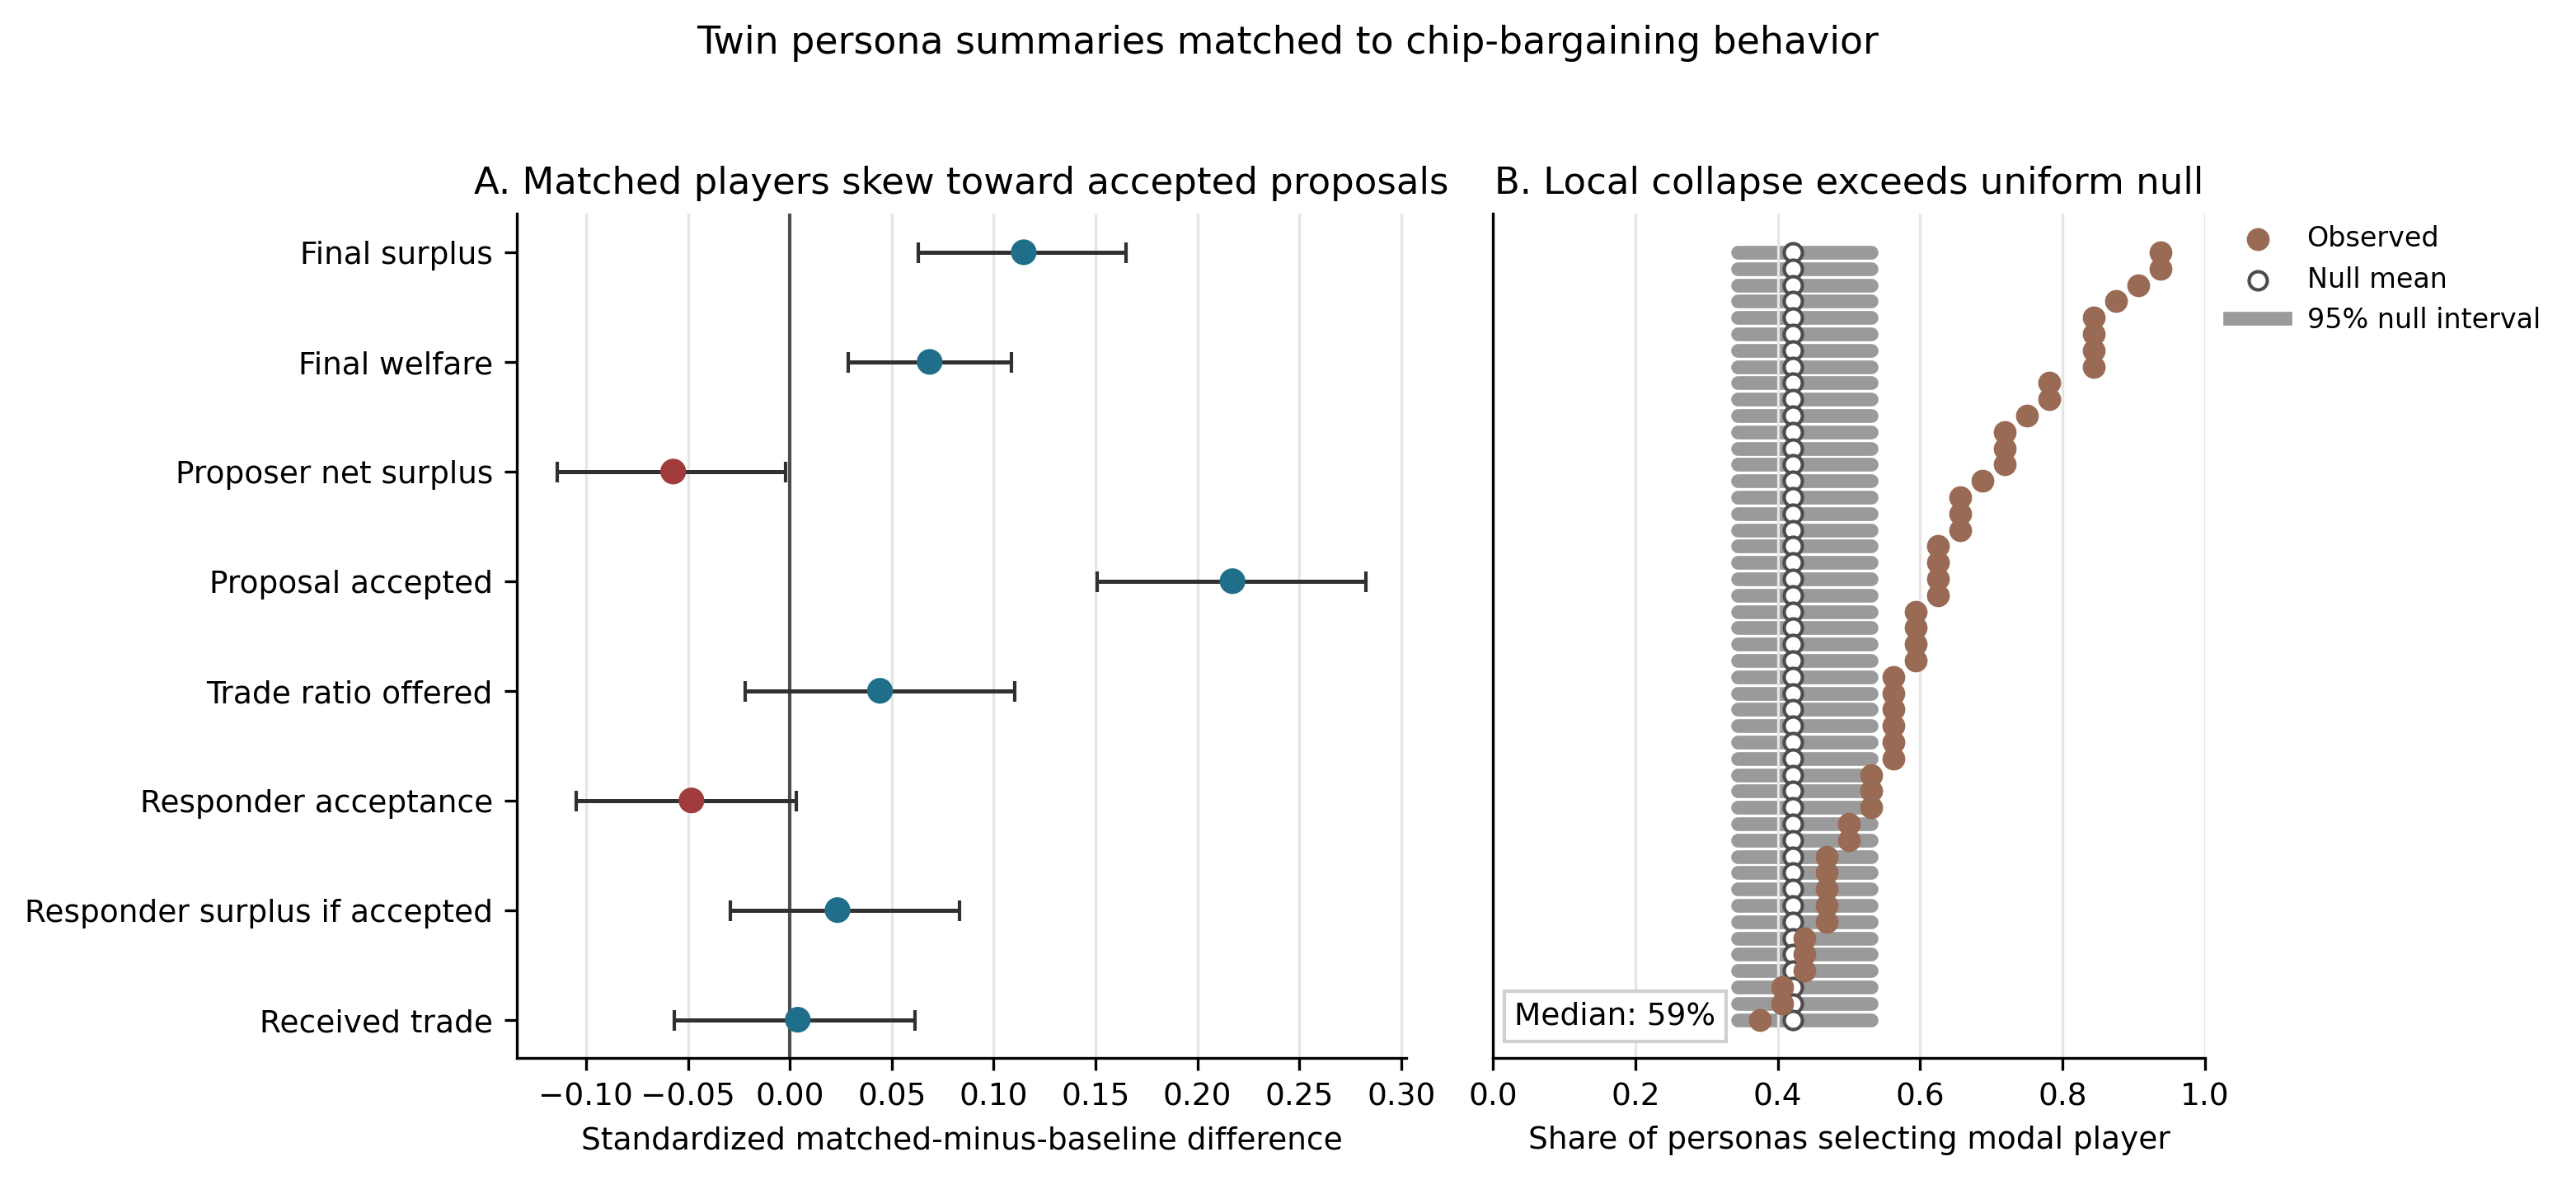
\includegraphics[width=\linewidth]{../figures/figure_chip_behavior_local_collapse.png}
\caption{\textbf{Chip-bargaining transfer evaluation.} Panel A reports probability-weighted matched-minus-candidate-uniform differences, divided by the candidate-uniform standard deviation for each bargaining metric. Error bars are 95 percent record-cluster bootstrap intervals. Panel B reports local concentration against the within-game uniform null: for each fixed three-player bargaining game, filled points show the observed modal top-1 share across personas, open points show the null mean, and gray intervals show 95 percent null intervals from uniform top-1 selection over the players in that game.}
\label{fig:chip-short}
\end{figure}

\subsection{Public Goods Games}

The PGG run crossed 32 Twin personas with 40 games, yielding 1,279 parsed requests. Local concentration was strong: the median modal player within a game received 54.0 percent of top-1 choices across personas. A within-game uniformity diagnostic rejected uniform top-1 selection in 39 of 40 games after Benjamini-Hochberg correction.

Global identity collapse was also strong (Figure 1). The model selected 200 of 342 candidate identities as top-1 at least once, or 58.5 percent. Under the request-conditional null, expected coverage was 93.6 percent. The observed entropy effective number was 38.5 percent of the candidate pool, compared with 75.1 percent under the null. The top 5 percent of identities received 29.0 percent of top-1 mass, compared with 16.1 percent under the null.

Matched players were behaviorally skewed. They contributed more, fully contributed more often, zero-contributed less often, varied less in their contributions, rewarded more, and received less punishment than the candidate-uniform baseline.

\subsection{Chip Bargaining}

The chip-bargaining run crossed 32 Twin personas with 48 three-player games, yielding 1,536 parsed requests. Local concentration was again visible: the median modal player within a game received 59.4 percent of top-1 choices, and uniform top-1 selection was rejected in 37 of 48 games after Benjamini-Hochberg correction.

Global identity collapse was milder than in PGG but still detectable. The model selected 135 of 144 candidate identities as top-1 at least once, or 93.8 percent. The request-conditional null expected essentially complete coverage. The observed entropy effective number was 73.2 percent of the candidate pool, compared with 96.8 percent under the null. The top 5 percent of identities received 14.6 percent of top-1 mass, compared with 8.4 percent under the null.

The behavioral skew was bargaining-specific. Matched players had higher final surplus and final welfare, and their proposals were accepted more often. At the same time, their proposer net surplus was slightly lower. Response-side metrics were weaker or unstable.

\section{Interpretation}

The evaluation separates failure modes that aggregate rollout accuracy would blur. PGG shows local concentration, strong global identity undercoverage, and cooperative/rewarding behavioral skew. Chip bargaining shows broader global coverage, but still non-uniform concentration and outcome-related skew. This suggests that persona libraries can fail to cover target behavior in different ways depending on the environment.

The central claim is not that Twin uniquely fails. The broader claim is that persona diversity in source space does not guarantee behavioral coverage in target-action space. Even when the model is allowed to choose among real human trajectories, a persona-library-plus-model system can map diverse personas to a narrowed and skewed subset of observed people.

\section{Next Analyses}

The next step is to vary both the persona source and the matcher model. We plan to compare direct Twin summaries with task-specialized Twin cards, demographic-only prompts, no-persona baselines, shuffled or placebo persona summaries, and generated persona libraries. Candidate external persona sources include persona generators that explicitly target support coverage \citep{paglieri2026persona}, as well as popular synthetic-persona generation pipelines used in survey simulation and agent-based modeling.

The no-persona baseline is especially important. It estimates the model's default attraction to particular observed behaviors. A useful persona library should improve behavioral coverage and reduce concentration relative to that default, not merely rename the model's preferred behavioral trace.

We also plan to extend the evaluation to additional multi-agent economic games and communication-rich settings. The most informative targets are games with both structured actions and transcripts, because they allow us to evaluate whether persona transfer preserves strategic behavior, interaction style, and communication patterns.

\bibliographystyle{apalike}
\bibliography{references}

\end{document}
